

\section{How to use the NSP}
\label{sec:NSP}


\section{C$_R$-based procedure}
\label{sec:CR}
\subsection{Theoretical background}
The aim of this procedure, proposed by Vamvatsikos (2014), is the estimation of the median spectral acceleration value $\hat{S}_{a,ds}$, that brings the structure to the attainment of a set of damage states ds, and the corresponding dispersion beta $\beta_{S_a}$, the parameters needed for the mathematical representation of fragility in equation \ref{eq:fragility-definition}. The aim is achieved making use of the work by Ruiz-Garcia and Miranda (2007), where the inelastic displacement demand is related to the elastic displacement with a simple relationship, and it can thus be easily estimated through a response spectrum analysis and a capacity curve.

The C$_R$-based procedure presented herein is applicable to bilinear elasto-plastic capacity curve only, and it is suitable for single building fragility curve estimation, as described in section \ref{subsubsec:single-building}. However the fragility curves derived for single buildings can be combined in a unique fragility curve, which considers the inter-building uncertainty, as described in section \ref{subsubsec:multiple-building}.

\subsubsection{Single Building Fragility and Vulnerability function}
\label{subsubsec:single-building}
This procedure provides a simple relationship between median damage state threshold, expressed in terms of top displacement $\delta_{roof}$, at each damage state threshold ds, and the corresponding median elastic Spectral displacement value $\hat{S}_{d,ds}(T_1)$.

\begin{equation}
\hat{\delta}_{roof, ds} = C_R S_{d, ds}(T_1) \Gamma_1 \Phi_1
\end{equation}

where $\Gamma_1 \Phi_1$ is the first mode participation factor estimated for the first-mode shape normalised by the roof displacement, and C$_R$ is the inelastic displacement ratio (inelastic over elastic spectral displacement), computed by Ruiz-Garcia and Miranda (2007) for nonlinear SDoF systems having hysteretic behaviour representative of the analysed structure, which is a function of the first-mode period of vibration and the relative lateral strength of the system R. Therefore the median Spectral acceleration at the fundamental period of vibration $\hat{S}_{a,ds}(T_1)$ turns out to be expressed as a function of the roof displacement according to the following equation:

\begin{equation}
\hat{S}_{a,ds}(T_1) = \frac{4 \pi^2}{\hat{C}_R T^2 \Gamma_1 \Phi_1} \hat{\delta}_{roof, ds}
\label{eq:Sa_RGM}
\end{equation}

Default values of $\hat{C}_R$ parameter estimates are provided by Ruiz-Garcia and Miranda (2007), as result of nonlinear regression analysis of three different measures of central tendency computed from 240 ground motions:

\begin{equation}
\hat{C}_R = 1 + \frac{R - 1}{79.12 T_1 ^{1.98}}
\label{eq:Cr_RGM}
\end{equation}

and values for R are given as:

\begin{equation}
R_{ds} = max(0.425(1 - c + \sqrt{c^2 + 2c(2 \mu_{ds} - 1) + 1}),1)
\label{eq:R_RGM}
\end{equation}

where c = 79.12 T$^{1.98}$, and $\mu_{ds}$ is the ductility at the damage state threshold of interest.

For what concerns the dispersion of $\hat{S}_{a,ds}$, $\beta_{S_a}$, the following relationship between S and the median EDP damage threshold $\hat{\theta}$ (Cornell, 2002) is used:

\begin{equation}
\hat{\theta}(S_a) = a S_a^b
\end{equation}

so that $\beta_{S_a}$ can be easily derived from the dispersion of $\theta$ due to record-to-record variability, $\beta_{\theta d}$, as in the following:

\begin{equation}
\beta_{S_a} = \frac{1}{b} \beta_{\theta d}
\label{eq:betaSa_RGM}
\end{equation}

The dispersion of $\theta$ due to record-to-record variability, $\beta_{\theta d}$ can be easily combined with the dispersion of $\theta$ due to uncertainty in the damage state threshold $\beta_{\theta c}$ as shown in the following equation:

\begin{equation}
\beta_{S_a} = \frac{1}{b} \sqrt{\beta_{\theta d}^2 + \beta_{\theta c}^2}
\label{eq:betaSc_RGM}
\end{equation}

The dispersion of $\theta$ can be obtained assuming that $d_{roof}$ and $\theta$ are proportional, and they thus share the same dispersion. Moreover the dispersion of $d_{roof}$ is the same as the dispersion of C$_R$, since they are also proportional. Finally $\beta_{\theta d}$ can be computed with the following equation, which represents Ruiz-Garcia and Miranda's (2007) estimate of C$_R$ dispersion:

\begin{equation}
\sigma_{\ln(C_R)} = \sigma_{\ln(d_{roof})} = \beta_{\theta d} =  1.975 [\frac{1}{5.876} + \frac{1}{11.749 (T + 0.1)}] [1- \exp(-0.739 (R - 1))]
\label{eq:beta_eq_RGM}
\end{equation}

To derive a discrete vulnerability function at certain intensity measure levels, the input damage-to-loss factors are applied to the probability of occurance of each damage state, extracted from the probability of exceedance of each damage state described by the fragility function. A value of loss ratio is thus defined for the vector of selected intensity measure levels.

\subsubsection{Multiple-Building Fragility and Vulnerability function}
\label{subsubsec:multiple-buildings}
If multiple buildings have been input to derive fragility function for a class of buildings all $\hat{S}_{a, blg}$ and $\beta_{S_a, blg}$ are combined in a single lognormal curve. A minimum of 5 buildings should be considered to obtain reliable results for the class. 
A new issue arises when multiple buildings are considered: the S$_a$ at the fundamental period of each building should be converted to a common intensity measure, to be able to combine the different fragility functions. A common intensity measure is selected to be S$_a$ at the period T$_{av}$, which is a weighted average of the individual buildings fundamental period T$_1$. Then each individual fragility needs to be expressed in terms of the common S$_a$(T$_{av}$), using a spectrum. FEMA P-695 far field set of 22 accelerograms was used to derive a mean uniform hazard spectrum, and the ratio between the S$_a$ at different periods is used to scale the fragility functions. It can be noted that the actual values of the spectrum are not important, but just the spectral shape. 
Median $\hat{S}_a$ is converted to the mean $\mu_{ln(S_a)}$ of the corresponding normal distribution ($\mu_{ln(S_a)} = ln(\hat{S}_a)$) and, simply scaled to the common intensity measure as follows:

\begin{equation}
\mu_{ln(S_a), blg} = \mu_{ln(S_a), blg} S(T_{av})/ S(T_{1, blg})
\end{equation}
\begin{equation}
\beta_{S_a, blg} = \beta_{S_a, blg} S(T_{av})/ S(T_{1, blg})
\label{eq:Sa(Tav)}
\end{equation}

Finally the parameters of the single lognormal curve for the class of buildings, mean and dispersion, can be computed as the weighted mean of the single means and the weighted SRSS of the inter-building and intra-building standard deviation, the standard deviation of the single means and the single dispersions respectively, as shown in the following equations:

\begin{equation}
\mu_{ln(S_a), tot} = \sum_{i=0}^{n.blg} w_{blg-i} \mu_{ln(S_a), blg-i}
\label{eq:combination-lognormals-mu}
\end{equation}
\begin{equation}
\beta_{S_a, tot} = \sqrt{ \sum_{i=0}^{n.blg} w_{blg-i} ((\mu_{ln(S_a), blg-i}-\mu_{ln(S_a), tot})^2+ \beta_{S_a, blg-i}^2})
\label{eq:combination-lognormals-sigma}
\end{equation}

The mean $\mu_{ln(S_a)}$ and total dispersion $\beta_{S_a}$ of the fragility function of the class are converted to logarithmic mean $\mu_{S_a}$ and logarithmic covariance $cov_{S_a}$ (standard deviation $\sigma_{S_a}$ over $\mu_{S_a}$), according to the following equations:

\begin{equation}
\hat{S}_a = e^{\mu_{ln(S_a)}}
\end{equation}
\begin{equation}
\mu_{S_a} = \hat{S}_a e^{\frac{\beta_{S_a}^2}{2}}
\label{eq:median-to-mean}
\end{equation}
\begin{equation}
\sigma_{S_a} = \sqrt[2]{(\beta_{S_a}^2-1) e^{2\ln{ \hat{S}_a}+\beta_{S_a}^2}}
\label{eq:dispersion-to-standard}
\end{equation}
\begin{equation}
cov_{S_a} = \frac{\sigma_{S_a}}{\mu_{S_a} }
\end{equation}

A single vulnerability function can be also obtained, from the single building vulnerability functions. The input damage-to-loss function is applied to the fragility function derived for each building. For the selected intensity measure levels a value of loss ratio $LR_{blg}$ is thus defined for each building. A discrete vulnerability function for the entire class of buildings is represented at each iml by a mean LR, $\mu_{LR,tot}$, equal tot the weighted $LR_{blg}$, and a standard deviation, $\sigma_{LR, tot}$, equal to the weighted standard deviation of all the computed $LR_{blg}$. The $\sigma_{LR, tot}$ of the fragility function of the class is converted to covariance $cov_{LR}$ (standard deviation $\sigma_{LR, tot}$ over $\mu_{LR, tot}$).

\subsection{Inputs}
\label{subsec:InputCr}
The inputs must be formatted as comma-separated value files (.csv), and saved in the folder \textit{input}, contained in the NSP directory. If any other environment different from Windows is used make sure that the "comma separated values Windows" is selected as saving option when creating the input files. 

If multiple buildings want to be analysed to consider the inter-building uncertainty the parameters relative to each building should be added as additional lines in the input tables, as shown in the examples below, otherwise a single line must be input.

If the user has already at disposal an idealised elasto-plastic pushover curve for each building, that is to say that the variable \textit{in\_type} has been set to 0, the following data need to be provided in the corresponding csv files:

\begin{enumerate}
\item First period of vibration T$_1$, corresponding modal participation factor $\Gamma_1$, normalised with respect to the roof displacement, and weight for the combination of different buildings, input in \textit{building\_parameters.csv}, as in the example below:
	\begin{table}[h]
	\centering
	\begin{tabular}{|c|c|c|c|} \hline
	\textbf{n.building} & \textbf{T$_1$} & \textbf{$\Gamma_1$} & \textbf{weights}\\ \hline
	1 & 0.32 & 1.23 & 0.2\\ \hline
	2 & 0.40 & 1.25 & 0.3\\ \hline
	... & ... & ... & ... \\ \hline
	\end{tabular}
	\end{table}
	
\item Roof displacement at each limit state LS and corresponding dispersion $\beta_{\theta c}$ input in \textit{displacement\_profile.csv}, as shown in the example below. If dispersion is unknown, $\beta_{\theta c}$ can be set equal to zero at each LS.
	\begin{table}[h]
	\centering
	\begin{tabular}{|c|c|c|c|} \hline
	\textbf{n.building} & \textbf{LS$_1$} &	\textbf{LS$_2$} &	\textbf{LS$_3$} \\ \hline
	1 & 0.066 & 0.169 & 0.23\\ \hline
	$\beta_{\theta d, 1}$ & 0.1 & 0.3 & 0.4\\ \hline
	2 & 0.08 & 0.172 & 0.25\\ \hline
	$\beta_{\theta d, 2}$ & 0.1 & 0.3 & 0.4\\ \hline	
	\end{tabular}
	\end{table}
	
\item Idealised pushover curve, input in \textit{idealised\_curve.csv} as shown below. The only required parameters are the yielding displacement $\delta_y$, the ultimate displacement $\delta_u$ and the yielding force F$_y$.

\begin{table}[h]
\centering
\begin{tabular}{|c|c|c|c|} \hline
\textbf{n.building} & \textbf{d$_y$} & \textbf{d$_u$} & \textbf{F$_y$} \\ \hline
1 & 0.09	& 0.3	 & 523\\ \hline
2 & 0.12	& 0.35	 & 400\\ \hline
... & ...	& ... & ...\\ \hline
\end{tabular}
\end{table}

\item Consequence model (loss ratio per each damage state) consistent with the defined set of damage states, input in \textit{consequence.csv}, as in the example below. A single consequence model can be input. This input is needed only if the variable \textit{vulnerability} has been set to 1.	
	\begin{table}[h]
	\centering
	\begin{tabular}{|c|c|c|} \hline
	\textbf{DS$_1$} & \textbf{DS$_2$} & \textbf{DS$_3$} \\ \hline
	0.2	& 0.5	 & 1\\ \hline
	\end{tabular}
	\end{table}
	
\end{enumerate}

If the idealised curve are not available, \textit{in\_type} = 0 can be selected and the displacements vs base shear at each time step results from a pushover analysis can be input instead. The following data need to be provided in the corresponding csv files:

\begin{enumerate}
\item T$_1$ and corresponding $\Gamma_1$, weight for the combination of different buildings, number of storeys and height of each storey, input in \textit{building\_parameters.csv}, as in the example below:
	\begin{table}[h]
	\centering
	\begin{tabular}{|c|c|c|c|c|c|c|c|c|} \hline
	\textbf{n.building} & \textbf{T$_1$} & \textbf{$\Gamma_1$} & \textbf{weights} & \textbf{n.Storey} & \textbf{H$_1$} & \textbf{H$_2$} & ... & \textbf{H$_n$} \\ \hline
	1 & 0.32 & 1.23 & 0.2 & 4 & 3 & 3 & ... & 3 \\ \hline
	2 & 0.40 & 1.25 & 0.3 & 4 & 4 & 2.7 & ... & 2.7 \\ \hline
	... & ... & ... & ... & ... & ... & ... & ... & ... \\ \hline
	\end{tabular}
	\end{table}
	
\item Displacements at each storey, at each incremental step of the pushover analysis, input in \textit{displacements\_pushover.csv}, as in the example below: 
	\begin{table}[h]
	\centering
	\begin{tabular}{|c|c|c|c|c|c|c|} \hline
	\textbf{n.building} & \textbf{n.Storey} & \textbf{Step1} & \textbf{Step 2} & \textbf{Storey 3} & ... & \textbf{Step n}\\ \hline
	1 &	1 & 0.0001 &	0.0005 &	0.001 & ... & 0.01\\ \hline
	   &	2 & 0.0003 &	0.0010 &	0.002 & ... & 0.02\\ \hline
	   &	3 & 0.0004 &	0.0016 &	0.003 & ... & 0.03\\ \hline
	   &	4 & 0.0006 &	0.0021 &	0.004 & ... & 0.04\\ \hline
	2 &	1 & 0.0001 &	0.0005 &	0.001 & ... & 0.01\\ \hline
	   &	2 & 0.0005 &	0.0012 &	0.002 & ... & 0.03\\ \hline
	   &	... & ... &	... &	... & ... & ...\\ \hline
	\end{tabular}
	\end{table}
	
\item Base shear at each incremental step of the pushover analysis input in \textit{reactions\_pushover.csv}, as in the example below:
	\begin{table}[h]
	\centering
	\begin{tabular}{|c|c|c|c|c|c|} \hline
	\textbf{n.building} &	\textbf{Step1} & \textbf{Step 2} & \textbf{Storey 3} & ... & \textbf{Step n} \\ \hline
	1 & 0.35 & 0.69 & 1.04 & ... & 29.12\\ \hline
	2 & 0.45 & 0.78 & 2.05 & ... & 40.00\\ \hline
	... & ... & ... & ... & ... & ...\\ \hline
	\end{tabular}
	\end{table}
	
\item Drift limit state and corresponding dispersion $\beta_{\theta c}$ input in \textit{limits.csv}. If dispersion is unknown, $\beta_{\theta c}$ can be set equal to zero at each limit state.
	\begin{table}[h]
	\centering
	\begin{tabular}{|c|c|c|c|} \hline
	\textbf{n.building} & \textbf{LS$_1$} &	\textbf{LS$_2$} &	\textbf{LS$_3$} \\ \hline
	1 & 0.01 &	0.025 & 0.0337\\ \hline
	$\beta_{\theta d, 1}$ &	0.1 & 0.2 & 0.25\\ \hline
	2 & 0.014 &	0.030 & 0.0430\\ \hline
	$\beta_{\theta d, 2}$ &	0.1 & 0.2 & 0.25\\ \hline
	\end{tabular}
	\end{table}

\item Consequence model (loss ratio per each damage state) consistent with the defined set of damage states, input in \textit{consequence.csv}, as in the example below. A single consequence model can be input. This input is needed only if the variable \textit{vulnerability} has been set to 1.
	\begin{table}[h]
	\centering
	\begin{tabular}{|c|c|c|} \hline
	\textbf{DS$_1$} & \textbf{DS$_2$} & \textbf{DS$_3$} \\ \hline
	0.2	& 0.5	 & 1\\ \hline
	\end{tabular}
	\end{table}
	
\end{enumerate}

\subsection{Calculation Steps}
The overall workflow of C$_R$-based procedure is summarised in this section. The option \textit{an\_type} must be set equal to 0 and the option \textit{in\_type} according to the input at disposal. The corresponding inputs should follow the requirements described in section \ref{subsec:InputCr}. At this point the code proceeds with the following steps:

\begin{enumerate}
\item
\begin{enumerate}
\item If \textit{in\_type} = 0 roof displacement at limit states and idealised pushover are extracted from \textit{displacement\_profile.csv} and \textit{idealised\_curve.csv} respectively.
\item If \textit{in\_type} = 1 results from pushover analysis are extracted from \textit{displacements\_pushover.csv} and \textit{reactions\_pushover.csv}, and drift limit states from \textit{limits.csv}. The idealised 	pushover curve is then derived in the \textit{idealisation} function, where the idealisation process is conducted according to FEMA-440. The elastic stiffness is defined as the 	tangent stiffness passing through the point of the pushover curve where 60\% of the maximum base shear is reached, and the perfectly plastic branch is set at an height equal to 	the maximum base shear. The yielding point is found as the interception between the elastic and the plastic branch.
\end{enumerate}

\item The csv input files are parsed with the function \textit{read\_data} according to the defined options. The parameters essential to the analysis are return together with a graphical visualisation of the inputs if the variable \textit{plotflag}[0] is equal to 1.

\item The parameters extracted are used in the \textit{simplified\_bilinear} function, within the \textit{fragility\_process} function, to derive ductility levels $\mu_{ds}$, median spectral acceleration $\hat{S}_{a,ds}$ and the total dispersion $\beta_{S_a}$ at each limit state through the following steps:
\begin{itemize}
\item The idealised MDoF system is transformed into an equivalent SDoF system, using $\Gamma_1$.
\item Ductility levels $\mu_{ds}$ corresponding to each damage threshold, are defined.
\item R and C$_R$ are computed, using eq. \ref{eq:R_RGM} and \ref{eq:Cr_RGM} respectively.
\item $\hat{S}_{a,ds}$ and the corresponding dispersion  $\beta_{\theta d}$ are computed using eq. \ref{eq:Sa_RGM} and \ref{eq:betaSa_RGM} respectively.
\item $\beta_{\theta d}$ is combined with dispersion due to uncertainty in the model $\beta_{\theta c}$, if different from zero, to get the total dispersion $\beta_{S_a}$, using eq. \ref{eq:betaSc_RGM}.
\item $\hat{S}_a(T_1)$ is converted to mean $\mu_{ln(S_a)}(T_1)$ and then to the intensity measure in common with the rest of the buildings, $\mu_{ln(S_a(T_{av}))}$, according to eq. \ref{eq:Sa(Tav)}
\end{itemize}

\item Step 3. is repeated for the number of input buildings.

\item
\begin{enumerate}
\item If vulnerability = 0: All $\mu_{ln(S_a), blg}$ and $\beta_{S_a, blg}$ are combined in a single lognormal curve, whose parameters are evaluated according to equations \ref{eq:combination-lognormals-mu} and \ref{eq:combination-lognormals-sigma}. Mean $\mu_{ln(S_{a})}$ and total dispersion $\beta_{S_a}$ are then converted to logarithmic mean $\mu_{S_a}$ and logarithmic covariance $cov_{S_a}$, according to equations \ref{eq:median-to-mean} and \ref{eq:dispersion-to-standard} respectively. Fragility curves for the class of buildings are displayed if the variable \textit{plotflag}[2] = 1, and logarithmic $\mu_{S_a}$ and $cov_{S_a}$ are exported in the \textit{outputs} folder.

\item If vulnerability =1: Vulnerability curves are derived for each fragility function derived at step 4. For the intensity measure levels defined in the variable \textit{iml} a value of loss ratio is thus defined for each building. They are finally combined in a single mean and its standard deviation, equal to the weighted mean and the weighted standard deviation of the loss ratios, as described in section \ref{subsec:InputCr}. Vulnerability curve for the class of buildings is displayed if the variable \textit{plotflag}[3] = 1. The $\sigma_{LR, tot}$ of the fragility function of the class is converted to covariance $cov_{LR}$ and $\mu_{LR}$ and $cov_{LR}$ at each iml are exported in the \textit{outputs} folder.
\end{enumerate}
\end{enumerate}

\section{Spo2ida-based procedure}
\label{sec:spo2ida}
\subsection{Theoretical background}
The aim of this procedure is the estimation of the median spectral acceleration value $\hat{S}_{a,ds}$, that brings the structure to the attainment of a set of damage states ds, and the corresponding dispersion beta $\beta_{S_a}$, the parameters needed for the mathematical representation of fragility in equation \ref{eq:fragility-definition}. The aim is achieved making use of the tool spo2ida (Vamvatsikos and Cornell, 2006), where static pushover curves are converted into 16\%, 50\% and 84\% IDA curves, using empirical relationships from a large database of incremental dynamic analysis results, as shown in Figure~\ref{fig:spo2ida}.

\begin{figure}[h]
\centering
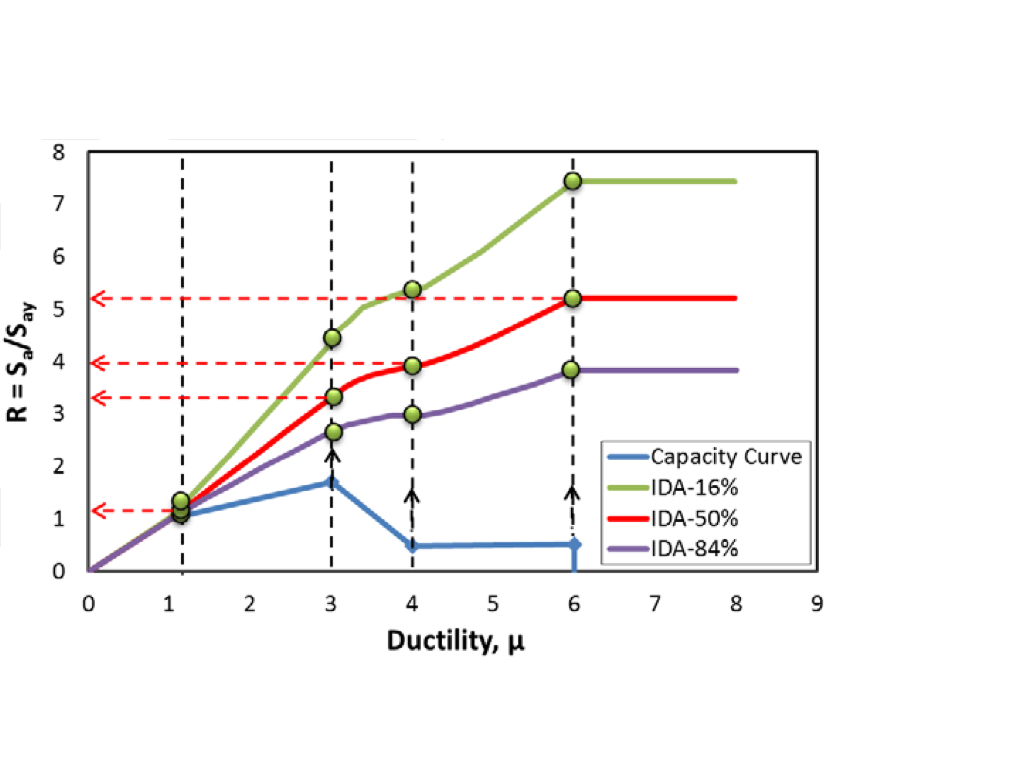
\includegraphics[width=12cm,height=8cm]{./figures/spo2ida.jpg}
\caption{spo2ida tool: IDA curves derived from Pushover curve.}
\label{fig:spo2ida}
\end{figure}

The spo2ida-based procedure presented herein is applicable to any kind of multi-linear capacity curve, and it is suitable for single building fragility curve estimation, as described in section \ref{subsubsec:single-building-spo2ida}. However the fragility curves derived for single buildings can be combined in a unique fragility curve, which considers the inter-building uncertainty, as described in section \ref{subsubsec:multiple-building-spo2ida}.

\subsubsection{Single-building Fragility and Vulnerability function}
\label{subsubsec:single-building-spo2ida}
Given the idealised capacity curve the spo2ida tool uses an implicit R-$\mu$-T relation to correlate nonlinear displacement, expressed in terms of ductility $\mu$ to the corresponding medians capacity in terms of the parameters R. R is the lateral strength ratio, defined as the ratio between the spectral spectral acceleration S$_a$ and the yielding capacity of the system S$_{ay}$. 

Each branch of the capacity curve, hardening, softening and residual plateau, is converted to a corresponding branch of the three ida curves, using the R-$\mu$-T relation, which is a function of the hardening stiffness, the softening stiffness and the residual force. These parameters are derived from the idealised pushover capacity expressed in $\mu$-R terms, as well as the ductility levels at the onset of each branch. If some of the branches of the pushover curve are missing because of the seismic behaviour of the system, spo2ida can equally work with bilinear, trilinear and quadrilinear idealisations.

The result of the spo2ida routine is thus a list of ductility levels and corresponding R values at 50\%, 16\% and 84\% percentiles. The distribution of R values at each ductility level, due to the record-to-record variability, is assumed to be lognormal and it can be easily converted to the dispersion of the lognormal distribution with the following equation:

\begin{equation}
\beta_{R(\mu)} = \frac{\ln R(\mu)_{84\%} - \ln R(\mu)_{16\%}}{2}
\label{eq:betaR}
\end{equation} 

$\beta_{R(\mu)}$ represents also the record-to-record variability of S$_a$ at different ductility levels $\beta_{S_a, d}$. Median R and its dispersion at ductility levels corresponding to the damage thresholds can thus be determined, and $\hat{S}_{a,ds}$ can be easily extracted simply multiplying $R_{50\%}(\mu_{ds})$ by the yielding capacity of the system $S_{ay}$, as shown in the following equation:

\begin{equation}
\hat{S}_{a,ds} = R_{50\%}(\mu_{ds}) S_{ay}
\label{eq:SaR}
\end{equation}
\begin{equation}
S_{ay} = \frac{4 \pi^2 \delta_{roof,y}}{g \Gamma_1 T_1^1}
\end{equation}

Since $\hat{R}$ and $\hat{S}_{a}$ are proportional they share the same dispersion.

If dispersion due to uncertainty in the limit state definition $\beta_{\theta c}$ is different from zero it can not be combined directly with the record-to-record dispersion, but a Monte Carlo sampling of the limit state needs to be performed instead. Different values of ductility limit state are sampled from the  lognormal distribution with median the median value of the ductility limit state, and dispersion the input $\beta_{\theta c}$. For each of these ductilities the corresponding R$_{16\%}$-R$_{50\%}$-R$_{84\%}$ are found and converted into $\hat{S}_{a,ds}$ and $\beta_{\theta d}$ according to equation \ref{eq:SaR} and \ref{eq:betaR}. N random S$_a$ corresponding to the N sampled ductility limit states are computed, and their median and the dispersion are estimated. These parameters constitute the median $\hat{S}_{a,ds}$ and the total dispersion $\beta_{S_a}$ for the considered damage state. The procedure is repeated for each damage state.

To derive a discrete vulnerability function at certain intensity measure levels, the input damage-to-loss factors are applied to the probability of occurance of each damage state, extracted from the probability of exceedance of each damage state described by the set of fragility curves. 

If dispersion due to uncertainty in the limit state is different from zero a vulnerability function is derived for the N sets of sampled ductility limit states. It results in N loss ratios for each defined intensity measure levels. Finally a lognormal distribution of the loss ratios is assumed at each iml and the vulnerability curve is defined at each iml by the mean and the standard deviation of all the computed loss ratios.

\subsubsection{Multiple-Building Fragility and Vulnerability function}
\label{subsubsec:multiple-building-spo2ida}
If multiple buildings have been input to derive a set of fragility curves for a class of buildings all $\hat{S}_{a,blg}$ and $\beta_{S_a,blg}$ are combined in a single lognormal curve for each damage state. A minimum of 5 buildings should be considered to obtain reliable results for the class. The procedure to get $\mu_{S_a,tot}$ and $cov_{S_a,tot}$ for the class of building is the same described in section \ref{subsubsec:multiple-buildings}, but the $\hat{S}_{a,blg}$ and $\beta_{S_a,blg}$ are those derived from each sampled set of ductility limit state.

A single vulnerability curve can also be obtained, from the single building vulnerability curves. If no dispersion in the limit state is defined, the method is the same described in section \ref{subsubsec:multiple-buildings}. Otherwise a vulnerability curve is derived for each building as explained in section \ref{subsub:single-building-spo2ida}, considering the sampled set of ductility limit states, that is to say that the mean loss ratio and its standard deviation at each iml, $\mu_{LR,iml,blg}$ and $\sigma_{LR,iml,blg}$ respectively, are found for each building.
Finally the mean loss ratio and its standard deviation, $\mu_{LR,iml}$ and $\sigma_{LR,iml}$, are found for the entire class of buildings as the weighted mean of the single $\mu_{LR,iml,blg}$ and the weighted SRSS of the inter-building and intra-building standard deviation, the standard deviation of the single means $\mu_{LR,iml,blg}$ and the single dispersions $\sigma_{LR,iml,blg}$ respectively, as described in eq \ref{eq:combination-lognormals-sigma}, substituting loss ratio to spectral acceleration.

\subsection{Inputs}
\label{subsec:InputSpo2ida}
The inputs must be formatted as comma-separated value files (.csv), and saved in the folder \textit{input}, contained in the NSP directory. If any other environment different from Windows is used make sure that the "comma separated values Windows" is selected as saving option when creating the input files. 

If multiple buildings want to be analysed to consider the inter-building uncertainty the parameters relative to each building should be added as additional lines in the tables, as shown in the examples below, otherwise a single line must be input.

If the user has already at disposal an idealised multilinear pushover curve for each building, that is to say that the variable \textit{in\_type} has been set to 0, the following data need to be provided in the corresponding csv files:

\begin{enumerate}
\item First period of vibration $T_1$, corresponding modal participation factor $\Gamma_1$, normalised with respect to the roof displacement, and weight for the combination of different buildings, input in \textit{building\_parameters.csv}, as in section \ref{subsec:InputCr}, input n. 1.
	
\item Top displacement at each damage state threshold and corresponding dispersion $\beta_{\theta c}$ input in \textit{displacement\_profile.csv}, as in section \ref{subsec:InputCr}, input n. 2. 
	
\item Idealised pushover curve, input in \textit{idealised\_curve.csv} as shown below. The parameters needed to describe the idealised pushover curve are: yielding displacement d$_y$, displacement at the onset of degradation d$_s$, displacement at the onset of residual force d$_{min}$, ultimate displacement d$_u$, maximum force F$_{max}$, residual force F$_{min}$. These parameters are represented in Figure~\ref{fig:quadrilinear}.

\begin{figure}[h]
\centering
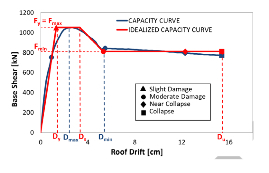
\includegraphics[width=12cm,height=8cm]{./figures/quadrilinear.jpg}
\caption{Idealisation of capacity curve using multilinear elasto-plastic form.}
\label{fig:quadrilinear}
\end{figure}

\begin{table}[h]
\centering
\begin{tabular}{|c|c|c|c|c|c|c|} \hline
\textbf{n.building} & \textbf{d$_y$} & \textbf{d$_s$} & \textbf{d$_{min}$} & \textbf{d$_u$} & \textbf{F$_{max}$} & \textbf{F$_{min}$} \\ \hline
1 & 0.09	& 0.3	& a & b & 523 & 430\\ \hline
2 & 0.12	& 0.35	 & a & b & 400 & 305\\ \hline	
\end{tabular}
\end{table}

\item Consequence model (loss ratio per each damage state) consistent with the defined set of damage states, input in \textit{consequence.csv}, as in section \ref{subsec:InputCr}, input n. 5.
	
\end{enumerate}

If these data are not available, \textit{in\_type} = 0 can be selected and the "raw" results from a pushover analysis can be input instead. The same data as in section \ref{subsec:InputCr} for \textit{in\_type} = 0 can be input.

\subsection{Calculation Steps}
The overall workflow of spo2ida-based procedure is summarised in this section. The option \textit{an\_type} must be set equal to 1 and the option \textit{in\_type} according to the input at disposal. The corresponding inputs should follow the requirements described in section \ref{subsec:InputSpo2ida}. At this point the code proceeds with the following steps:

\begin{enumerate}
\item 
\begin{enumerate}
\item If \textit{in\_type} = 0, the roof displacement at each limit state and the idealised pushover curve parameters are extracted from \textit{displacement\_profile.csv} and \textit{idealised\_curve.csv} respectively.

\item If \textit{in\_type} = 1 the results from a pushover analysis are extracted from \textit{displacements\_pushover.csv} and \textit{reactions\_pushover.csv} and drift limit states from {limits.csv}. The idealised pushover curve is then derived in the \textit{idealisation} function, where the idealisation process is conducted according to the Gem Analytical Vulnerability Guidelines.	\end{enumerate}

\item The parameters extracted are used to derive ductility levels $\mu_{ds}$, median spectral acceleration $\hat{S}_{a,ds}$ and the total dispersion $\beta_{S_a}$ at each damage threshold through the following steps:
\begin{itemize}
\item The idealised MDoF system is transformed into an equivalent SDoF system, using $\Gamma_1$, and SDoF capacity curve is  expressed in terms of $\mu$-R.

\item The variables for spo2ida tool are extracted from the capacity curve and they are used as input to get the 16\%-50\%-84\% ida curves.

\item The ductility levels $\mu_{ds}$ corresponding to each damage threshold are defined, and the corresponding R$_{16\%}$-R$_{50\%}$-R$_{84\%}$ are found in ida outputs.

\item $\hat{S}_{a,ds}$ and the corresponding dispersion $\beta_{S_{a, d}}$ are computed using eq.~\ref{eq:SaR} and eq.~\ref{eq:betaR}, respectively.

\item If dispersion due to uncertainty in the limit state $\beta_{\theta c}$ is different from zero different ductility limit states are sampled for each median ductility level $\mu_{ds}$ and corresponding values of $\hat{S}_{a,ds}$ and $\beta_{S_{a, d}}$ are computed, as described in section \ref{subsubsec:single-building-spo2ida}, but not yet combined together.

\end{itemize}

\item All $\hat{S}_{a, ds}(T_1)$ are converted to mean $\mu_{ln(S_{a, ds})}(T_1)$ and then to the intensity measure in common with the rest of the buildings, $\mu_{ln(S_{a, ds}(T_{av}))}$, according to eq. \ref{eq:Sa(Tav)}.

\item Step 2. and 3. are repeated for the number of input buildings.

\item
\begin{enumerate}

\item If vulnerability = 0: All $\hat{S}_{a,ds}$ and $\beta_{S_{a, d}}$ from all the buildings and all the sampled ductility limit states are combined in a single lognormal curve, as described in section \ref{subsub:single-building-spo2ida}. 
Mean $\mu_{ln(S_{a})}$ and total dispersion $\beta_{S_a}$ are then converted to logarithmic mean $\mu_{S_a}$ and logarithmic covariance $cov_{S_a}$, according to equations \ref{eq:median-to-mean} and \ref{eq:dispersion-to-standard} respectively.
Fragility curves for the class of buildings are displayed if the variable \textit{plotflag}[2] = 1, and logarithmic $\mu_{S_a}$ and $cov_{S_a}$ are exported in the \textit{outputs} folder.
\item If vulnerability =1:  
For the intensity measure levels defined in the variable \textit{iml} a value of loss ratio $\mu_{LR, iml, blg}$ is defined for each building and a standard deviation $\sigma_{LR, iml, blg}$, if dispersion due to uncertainty in the limit state $\beta_{\theta c}$ is different from zero. They are finally combined in a single mean and standard deviationas described in section \ref{multiple-building-spo2ida}. Vulnerability curve for the class of buildings is displayed if the variable \textit{plotflag}[3] = 1, and $\mu_{LR}$ and $cov_{LR}$ at each iml are exported in the \textit{outputs} folder.
\end{enumerate}

\end{enumerate}

\section{R-$\mu$-T procedure}
\label{sec:DF}
\subsection{Theoretical background}
The aim of this procedure is the estimation of the median spectral acceleration value $\hat{s}_c$, that brings the structure to the attainment of a set of damage states, and the corresponding dispersion beta $\beta_{sc}$, the parameters needed for the mathematical representation of fragility in equation \ref{eq:fragility-definition}. The aim is achieved making use of a R-$\mu$-T relationship, between the reduction factor R, the ductility $\mu$ and period T, which is based on the work of Dolsek and Fajfar (2004). The R-$\mu$-T-based procedure presented herein is applicable to any kind of multi-linear capacity curve, and it is suitable for single building fragility curve estimation, as described in section \ref{subsubsec:single-building-DF}. However the fragility curves derived for single buildings can be combined in a unique fragility curve, which considers the inter-building uncertainty, as described in section \ref{subsubsec:multiple-building-DF}.

\subsubsection{Single Building Fragility and Vulnerability function}
\label{subsubsec:single-building-DF}
The spectral value at each damage state threshold ds $\hat{S}_{a,ds}$ is found from the top displacement representing that ds attainment $\hat{\delta}_{roof, ds}$, as explained in C$_{R}$\_based procedure and reported the following equation:

\begin{equation}
\hat{S}_{a,ds}(T_1) = \frac{4 \pi^2}{\hat{C}_R T^2 \Gamma_1 \Phi_1} \hat{\delta}_{roof, ds}
\label{eq:basic_DF}
\end{equation}

The value of C$_R$, the ratio between the inelastic and the elastic spectral displacement, is found from equation \ref{eq:Cr_DF}.

\begin{equation}
\hat{C}_{R} = \frac{\mu_{LS}}{R_{LS}}
\label{eq:Cr_DF}
\end{equation}

where $\mu_{ds}$ and $R_{ds}$ are the ductility level and the reduction factor at each ds attainment. According to the results of an extensive parametric study using three different sets of recorded and semi-artificial ground motions Dolsek and Fajfar (2004) related the ductility demand, $\mu$ , and reduction factor, R , through the following formula:

\begin{equation}
\label{eq:mu_DF}
\mu = \frac{1}{c} (R-R_{0})+\mu_{0}
\end{equation}

In the proposed model, $\mu$ is linearly dependent on R within two reduction factor intervals. The parameter c defines the slope of the R–$\mu$ relation, and depends on the initial period of the system T, the ratio r$_{u}$, the reduction factor R and the corner periods T$_{c}$ and T$_{d}$. T$_{c}$ and T$_{d}$ are the corner periods between the constant acceleration and constant velocity part of the idealized elastic spectrum, and between the constant velocity and constant displacement part of the idealized elastic spectrum respectively.

Given the parameters of the multilinear pushover curves (R$_{\mu_{c}}$, $\mu_{c}$, r$_{u}$) and T, the median R-$\mu$ curve, similar to an IDA curve, can be construct using the aforementioned relationship.  A multilinear capacity curve and the corresponding R$_{\mu_{c}}$, $\mu_{c}$ and r$_{u}$ parameters are shown in Figure \ref{fig:quadrilinear_DF}.

\begin{figure}[h]
\centering
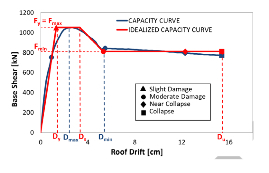
\includegraphics[width=10cm,height=5cm]{./figures/quadrilinearDF.jpg}
\caption{Multilinear capacity curve and parameters for the definition of R-$\mu$ relation.}
\label{fig:quadrilinear_DF}
\end{figure}

On the median "IDA curve" the $\mu$-R pairs corresponding to the limit states (R$_{LS}$ and $\mu_{LS}$) can be found and turned into median spectral acceleration values for that limit state $\hat{S}_c$, to be used in equation \ref{eq:basic_DF}.

Once median R$_{LS}$ and $\mu_{LS}$ are found, the 84 and 16 fractiles $\mu$ are extracted using top drift record-to-record dispersion $\sigma_{ln(\delta)}$ from equation \ref{eq:beta_eq_RGM}, by Ruiz-Garcia and Miranda (2007). The steps to derive $\mu_{16}$ and $\mu_{84}$ are the following:
 
\begin{equation}
ln(\delta)_{16} = ln(\hat{\delta})-\sigma_{ln(\delta)}
\end{equation}
\begin{equation}
ln(\delta)_{84} = ln(\hat{\delta})+\sigma_{ln(\delta)}
\end{equation}
\begin{equation}
\mu_{16} = \hat{\mu} \exp{-\sigma_{ln(\delta)}}
\end{equation}
\begin{equation}
\mu_{84} = \hat{\mu} \exp{\sigma_{ln(\delta)}}
\end{equation}

Given the linear relationship between R and $\mu$, the R$_{16}$ and R$_84$ values at $\mu_{LS}$ are just linearly interpolated, and the record-to-record dispersion of the spectral acceleration $\beta_{S_{a, d}}$ at each $\mu_{LS}$ coincides with the dispersion of R, computed from the percentiles values.

\begin{equation}
\label{eq:beta_DF}
\beta_{R(\mu)} = \frac{\ln R(\mu)_{84\%} - \ln R(\mu)_{16\%}}{2}
\end{equation} 

The dispersion of $S_{a}$ due to uncertainty in the damage state threshold $\beta_{S_{a, c}}$ can be found converting the dispersion on the damage threshold $\beta_{\theta c}$, as explaind in equation \ref{eq:betaSa_RGM} and reported in the following equation.

\begin{equation}
\label{eq:betasc_DF}
\beta_{S_{a, c}} = \frac{1}{b} \beta_{\theta c}
\end{equation}

In order to derive the b values, which represent the slope of the R-$\mu$ relation in the log-space, a further step needs to be made, because the R-$\mu$-T is suggested by the authors as conservative, since it is not based on the median but on the mean $\mu$ given R. An attempt was made to correct b reducing the median R curve by 15\%, $\hat{R}_{corrected}$, and extrapolating the corresponding $\hat{\mu}_{corrected}$.

\begin{equation}
\hat{R}_{corrected}=0.85\hat{R}
\end{equation}
\begin{equation}
\label{eq:bcorrected_DF}
b=ln(\hat{\mu}_{corrected})/ln(\hat{R}_{corrected})
\end{equation}

Finally the dispersion of $S_{a}$ due to record-to-record variability, $\beta_{S_{a, d}}$ can be easily combined with the dispersion of $S_{a}$ due to uncertainty in the damage state threshold $\beta_{S_{a, c}}$ as shown in the following equation.

\begin{equation}
\label{eq:betatotal_DF}
\beta_{S_a} = \sqrt{\beta_{S_{a, c}}^2 + \beta_{S_{a, d}}^2}
\end{equation}

\subsubsection{Multiple Building Fragility and Vulnerability function}
\label{subsubsec:multiple-building-DF}
 If multiple buildings have been input to derive fragility function for a class of buildings all $\hat{S}_{a, blg}$ and $\beta_{S_a, blg}$ are combined in a single lognormal curve as described in section \ref{subsubsec:multiple-buildings}. The same holds for vulnerability function, as described in the same section.

\subsection{Inputs}
The data the user needs provided and the their format is described in section \ref{subsec:InputSpo2ida}

\subsection{Calculation Steps}
The overall workflow of R-$\mu$-T-based procedure is summarised in this section. The option \textit{an\_type} must be set equal to 2 and the option \textit{in\_type} according to the input at disposal. The corresponding inputs should follow the requirements described in section \ref{subsec:InputSpo2ida}. At this point the code proceeds with the following steps:

\begin{enumerate}
\item 
\begin{enumerate}
\item If \textit{in\_type} = 0, the roof displacement at each limit state and the idealised pushover curve parameters are extracted from \textit{displacement\_profile.csv} and \textit{idealised\_curve.csv} respectively.

\item If \textit{in\_type} = 1 the results from a pushover analysis are extracted from \textit{displacements\_pushover.csv} and \textit{reactions\_pushover.csv} and drift limit states from {limits.csv}. The idealised pushover curve is then derived in the \textit{idealisation} function, where the idealisation process is conducted according to the Gem Analytical Vulnerability Guidelines.	\end{enumerate}

\item The csv input files are parsed with the function \textit{read\_data} according to the defined options. The parameters essential to the analysis are return together with a graphical visualisation of the inputs if the variable \textit{plotflag}[0] is equal to 1.

\item The parameters extracted are used in the \textit{DFfragility} function, within the \textit{fragility\_process} function, to derive ductility levels $\mu_{ds}$, median spectral acceleration $\hat{S}_{a,ds}$ and the total dispersion $\beta_{S_a}$ at each limit state through the following steps:
\begin{itemize}
\item The idealised MDoF system is transformed into an equivalent SDoF system, using $\Gamma_1$.
\item Ductility levels $\mu_{ds}$ corresponding to each damage threshold, are defined.
\item R and C$_R$ are computed, using eq. \ref{eq:mu_DF} and \ref{eq:Cr_DF} respectively.
\item $\hat{S}_{a,ds}$ and the corresponding dispersion  $\beta_{\S_{a, d}}$ are computed using eq. \ref{eq:basic_DF} and \ref{eq:beta_DF} respectively.
\item R$_{corrected}$ curve are found reducing by 15\% the median R curve, and the corresponding $\mu_{corrected}$ corrected are extrapolated.
\ b value is found from R and mu according to eq. \ref{eq:bcorrected_DF}.
\item Uncertainty in the model is expressed in terms of dispersion in S$_a$ $\beta_{\S_{a, c}}$ according to eq. \ref{eq:betasc_DF} and combined with $\beta_{\S_{a, d}}$ to get the total dispersion $\beta_{S_a}$, using eq. \ref{eq:betatotal_DF}.
\item $\hat{S}_a(T_1)$ is converted to mean $\mu_{ln(S_a)}(T_1)$ and then to the intensity measure in common with the rest of the buildings, $\mu_{ln(S_a(T_{av}))}$, according to eq. \ref{eq:Sa(Tav)}
\end{itemize}

\item Step 3. is repeated for the number of input buildings.

\item
\begin{enumerate}
\item If vulnerability = 0: All $\mu_{ln(S_a), blg}$ and $\beta_{S_a, blg}$ are combined in a single lognormal curve, whose parameters are evaluated according to equations \ref{eq:combination-lognormals-mu} and \ref{eq:combination-lognormals-sigma}. Mean $\mu_{ln(S_{a})}$ and total dispersion $\beta_{S_a}$ are then converted to logarithmic mean $\mu_{S_a}$ and logarithmic covariance $cov_{S_a}$, according to equations \ref{eq:median-to-mean} and \ref{eq:dispersion-to-standard} respectively. Fragility curves for the class of buildings are displayed if the variable \textit{plotflag}[2] = 1, and logarithmic $\mu_{S_a}$ and $cov_{S_a}$ are exported in the \textit{outputs} folder.

\item If vulnerability =1: Vulnerability curves are derived for each fragility function derived at step 4. For the intensity measure levels defined in the variable \textit{iml} a value of loss ratio is thus defined for each building. They are finally combined in a single mean and its standard deviation, equal to the weighted mean and the weighted standard deviation of the loss ratios, as described in section \ref{subsec:InputCr}. Vulnerability curve for the class of buildings is displayed if the variable \textit{plotflag}[3] = 1. The $\sigma_{LR, tot}$ of the fragility function of the class is converted to covariance $cov_{LR}$ and $\mu_{LR}$ and $cov_{LR}$ at each iml are exported in the \textit{outputs} folder.
\end{enumerate}

\end{enumerate}